\section{Diverses}

\subsection{Von $G(s)$ zur DGL}
  \begin{multicols}{2}
    \begin{itemize}
      \item $G(s)$ als Bruch aufschreiben.
			\item Zähler = Eingang ($u$) \quad Nenner = Ausgang ($y$)
 			\item $j\omega = \dot{y} \quad (j\omega)^2 = \ddot{y} \quad \ldots $
 			\item Gleiches gillt für den Zähler mit u!
		\end{itemize}
	\columnbreak
		\textbf{Beispiel:} $G(s) = \frac{K(j \omega T + 1)}{(j\omega)^2 T_N + j \omega Tn(1+K_R) + K_R}$ \\			
		\textbf{DGL:} $T_N \ddot{y} + T_N(1+K_R) \dot{y} + K_R y = K(T \dot{u} + u)$
  \end{multicols}    	
    
\subsection{Zeigerdiagramme}
  Soll zu einem gegebenen Blockschaltbild (oder einer gegebenen Funktion) das Zeigerdiagramm erstellt 
  werden, werden die \textbf{Beträge} der Elemente \textbf{multipliziert} und
  die \textbf{Winkel} ($arg()$) \textbf{addiert}. Die Werte für die einzelnen Elemente sind der Tabelle in Kap.\ref{subsec:LTI-Grundglieder} \nameref{subsec:LTI-Grundglieder} zu entnehmen. 

\begin{multicols}{2}
  \subsection{Graphisch Phasen-/Verstärkungsreserve}
    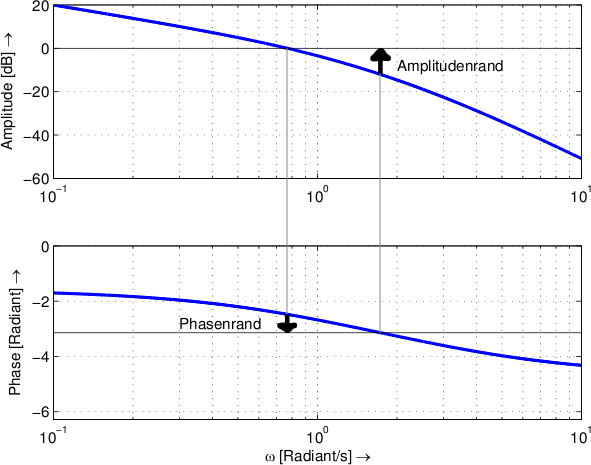
\includegraphics[width=7cm]{./images/bode-stabilitaet.png} \\
    Phasen-/Verstärkungsreserve = Phasen-/Amplitudenrand
    
\columnbreak

  \subsection{Störgrössenaufschaltung \formelbuch{204}}
    Bei der Störgrössenaufschaltung wird auch die Hauptstörung (Last) gemessen und verarbeitet.\\
    \textbf{Merkmale:}
    \begin{itemize}[leftmargin=*]
      \item Hauptstörung wird früher erkannt, was die Regelgeschwindigkeit stark verbessert.
      \item Für die Genauigkeit sorgt weiterhin der Regelkreis. Weitere Störungen werden damit auskorrigiert.
      \item Das Führungsverhalten wird durch die Störgrössenaufschaltung nicht beeinflusst. Somit auch nicht
            die Stabilität der Regelung.
      \item Die Zeitverzögerung zwischen Störort und Aufschaltort soll gering sein.
    \end{itemize}
\end{multicols}

\subsection{Kaskadenregelung \formelbuch{205}}
  Die Kaskadenregelung besitzt einen oder mehrere unterlagerte Regelkreise.\\
  \begin{itemize}
    \item Die Hauptstörung, welche oft am Anfang der Strecke angreift, wird rascher erkannt und kann
          schneller auskorrigiert werden.
    \item Die Dynamik wird verbessert.
    \item Die positiven Nebenwirkungen der inneren Regelung, wie Linearisierung der Strecke
          und Reduktion der Parameterempfindlichkeit, sind erwünscht.
    \item Die Kaskadenregelung vereinfacht die Regler und erleichtert ihre Einstellung.
  \end{itemize}

\subsection{diskreter PID \formelbuch{244}}
  Grundaufgaben eines diskreten PID:
  \begin{itemize}
    \item Erfassen der Regelgrösse über die Messeinrichtung (AD-Wandlung)
    \item Fehler bestimmen durch Vergleich
    \item Korrektur berechnen
    \item Korrektur am Prozess über die Stelleinrichtung vornehmen (DA-Wandlung)
  \end{itemize}

\section{Umformungen}
 \begin{multicols}{2}
	\subsection{Serielle Systeme}
		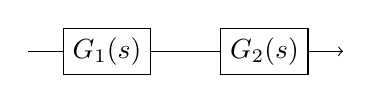
\begin{tikzpicture}
  \node (G1) at (1,0) [draw]{$G_1(s)$};

  \node (G2) at (3,0) [draw]{$G_2(s)$};

  \draw [->] (0,0) --  (node cs:name=G1) --  (node cs:name=G2)  -- ++(1,0);
\end{tikzpicture}


		$G(s) = G_1(s) \cdot G_2(s)$
	\subsection{Parallele Systeme}
		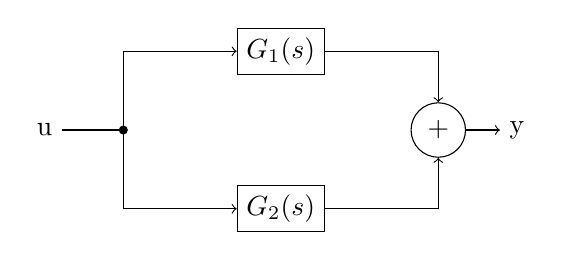
\begin{tikzpicture}
  \node (in) at (0,1) []{u};
  \node (dot) at (1,1) [draw,circle,inner sep=1,fill]{};

  \node (G1) at (3,2) [draw]{$G_1(s)$};
  \node (G2) at (3,0) [draw]{$G_2(s)$};

  \node (sum) at (5,1) [circle,draw]{+};
  \node (out) at (6,1) []{y};


  \draw (in) -> (dot);
 
  \draw[->] (dot) |-  (G1);
  \draw[->] (G1) -| (sum);

  \draw[->] (dot) |-  (G2);
  \draw[->] (G2) -| (sum);

  \draw[->](sum) -- (out);

\end{tikzpicture}


		$G(s) = G_1(s) + G_2(s)$
	\subsection{Zwei Systeme mit Rückkopplung}
		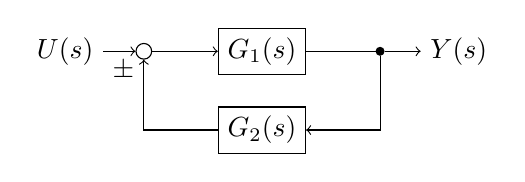
\begin{tikzpicture}
  \node (in) at (0,2) []{$U(s)$};
  \node (sum) at (1,2) [circle,draw,inner sep=2]{};
  \node (G1) at (2.5,2) [draw]{$G_1(s)$};
  \node (G2) at (2.5,1) [draw]{$G_2(s)$};
  \node (dot) at (4,2) [draw,circle,inner sep=1,fill]{};
  \node (out) at (5,2) []{$Y(s)$};

  \node (feedback) at (sum) [below left] {$\pm$};

  \draw[->] (in) -- (sum);
  \draw[->] (sum) --  (G1);
  \draw (G1) --  (dot);
  \draw[->](dot) -- (out);

  \draw[->] (dot) |-(G2);
  \draw[->] (G2) -| (sum);

\end{tikzpicture}

\newline
		$G(s) = \frac{G_1(s)}{1 \mp G_1(s) G_2(s)}$ Vorzeichenwechsel! \\
		
		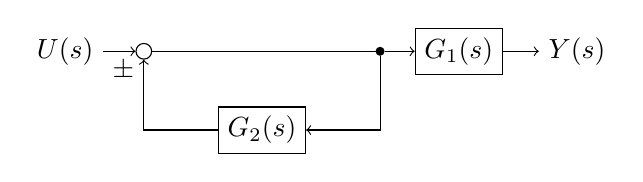
\begin{tikzpicture}
  \node (in) at (0,2) []{$U(s)$};
  \node (sum) at (1,2) [circle,draw,inner sep=2]{};
  \node (G1) at (5,2) [draw]{$G_1(s)$};
  \node (G2) at (2.5,1) [draw]{$G_2(s)$};
  \node (dot) at (4,2) [draw,circle,inner sep=1,fill]{};
  \node (out) at (6.5,2) []{$Y(s)$};

  \node (feedback) at (sum) [below left] {$\pm$};

  \draw[->] (in) -- (sum);
  \draw (sum) --  (dot);
  \draw[->] (dot) --  (G1);
  \draw[->](G1) -- (out);

  \draw[->] (dot) |-(G2);
  \draw[->] (G2) -| (sum);

\end{tikzpicture}
\newline
		$G(s) = G_1(s) \cdot \frac{1}{1 \mp G_2(s)}$ Vorzeichenwechsel!
		
  \end{multicols}
	\subsection{Komplexeres Beispiel}
		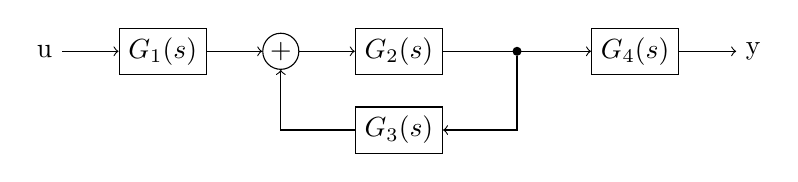
\begin{tikzpicture}
  \node (in) at (0,2) []{u};
  \node (G1) at (1.5,2) [draw]{$G_1(s)$};

  \node (sum) at (3,2) [circle,draw,inner sep=1]{+};

  \node (G2) at (4.5,2) [draw]{$G_2(s)$};
  \node (G3) at (4.5,1) [draw]{$G_3(s)$};

  \node (dot) at (6,2) [draw,circle,inner sep=1,fill]{};
  \node (G4) at (7.5,2) [draw]{$G_4(s)$};
  \node (out) at (9,2) []{y};


  \draw[->] (in) -- (G1);
 
  \draw[->] (G1) --  (sum);
  \draw[->] (sum) --  (G2);

  \draw (G2) -- (dot);
  \draw[->] (dot) |-(G3);
  \draw[->] (G3) -| (sum);

  \draw[->] (dot) |-  (G4);
  \draw[->](G4) -- (out);

\end{tikzpicture}


		$G(s) = G_1(s) \cdot \frac{G_2(s)}{1-G_2(s) \cdot G_3(s)} \cdot G_4(s)$


\begin{landscape}
\subsection{Approximation des Bode-Diagramms}
\renewcommand{\arraystretch}{1.5}
\begin{longtable}{|p{5cm}|l|ll|ll|}
	\hline
		\textbf{Pole} & 
		\textbf{UTF} $H(s)$ &
		\multicolumn{2}{c}{\textbf{Amplitude} $|H(s)|$} & 
		\multicolumn{2}{|c|}{\textbf{Phase} $\angle(H(s))$}
	\\ \hline
		Keine, konstanter Faktor &
		$\alpha e^{j \beta}$ &
		\parbox[c][1cm]{1cm}{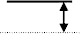
\includegraphics[width=1cm]{./images/bode-approx-konst.png}} &
		\, Konstant: $20 \log \alpha$ &
		\parbox[c][1cm]{1cm}{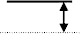
\includegraphics[width=1cm]{./images/bode-approx-konst.png}} &
		Konstant: $\beta$
	\\ \hline
		Pol im Ursprung &
		$\frac{\alpha}{s}$ &
		\parbox[c][1cm]{1cm}{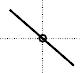
\includegraphics[width=1cm]{./images/bode-approx-ampl-tp-ord1.png}} & 
		\begin{tabular}{l}
			Lineare Steigung: $-20 dB/Dek.$ \\
			$0dB$ bei $\omega = \alpha$
		\end{tabular} &
		\parbox[c][1cm]{1cm}{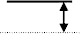
\includegraphics[width=1cm]{./images/bode-approx-konst.png}} & 
		Konstant: $-\frac{\pi}{2}$ 
	\\ \hline
		Nullstelle im Ursprung &
		$\alpha s$ &
		\parbox[c][1cm]{1cm}{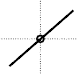
\includegraphics[width=1cm]{./images/bode-approx-ampl-hp-ord1.png}} & 
		\begin{tabular}{l}
			Lineare Steigung: $+20 dB/Dek.$ \\
			$0dB$ bei $\omega = \frac{1}{\alpha}$
		\end{tabular} &
		\parbox[c][1cm]{1cm}{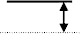
\includegraphics[width=1cm]{./images/bode-approx-konst.png}} &
		Konstant: $+\frac{\pi}{2}$
	\\ \hline	
		Reeller Pol &
		$\frac{1}{s + \alpha}$ &
		\parbox[c][1cm]{1cm}{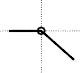
\includegraphics[width=1cm]{./images/bode-approx-ampl-4.png}} &
		\begin{tabular}{ll}
			$\omega < \alpha$: & Konstant $-20 \log \alpha$  \\
			$\omega > \alpha$: & $-20dB/Dek.$
		\end{tabular} &
		\parbox[c][1cm]{1cm}{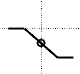
\includegraphics[width=1cm]{./images/bode-approx-phase-4.png}} &
		\begin{tabular}{ll}
			$\omega < \frac{\alpha}{10} $:	& Konstant $0$ \\
			$\omega > 10 \alpha$:		& Konstant $-\frac{\pi}{2}$
		\end{tabular}
	\\ \hline
		Reeller Pol &
		$\frac{\alpha}{s + \alpha}$ &
		\parbox[c][1cm]{1cm}{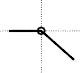
\includegraphics[width=1cm]{./images/bode-approx-ampl-4.png}} &
		\begin{tabular}{ll}
			$\omega < \alpha$: & Konstant $0dB$ \\
			$\omega > \alpha$: & $-20dB/Dek. \qquad (\omega_r = \alpha)$
		\end{tabular} &
		\parbox[c][1cm]{1cm}{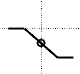
\includegraphics[width=1cm]{./images/bode-approx-phase-4.png}}	& 
		\begin{tabular}{ll}
			$\omega < \frac{\alpha}{10}$: & Konstant $0$ \\
			$\omega > 10 \alpha$: & Konstant $-\frac{\pi}{2}$
		\end{tabular}
	\\ \hline
		Reelle Nullstelle &
		$s + \alpha$ & 
		\parbox[c][1cm]{1cm}{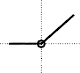
\includegraphics[width=1cm]{./images/bode-approx-ampl-5.png}} &
		\begin{tabular}{ll}
			$\omega < \alpha$: & Konstant $20 \log \alpha$ \\
			$\omega > \alpha$: & $+20dB/Dek.$
		\end{tabular} & 
		\parbox[c][1cm]{1cm}{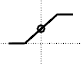
\includegraphics[width=1cm]{./images/bode-approx-phase-5.png}}	&
		\begin{tabular}{ll}
			$\omega < \frac{\alpha}{10}$: & Konstant $0$ \\
			$\omega > 10 \alpha$: & Konstant $+\frac{\pi}{2}$
		\end{tabular}
	\\ \hline	
		Reelle Nullstelle &
		$\frac{s + \alpha}{\alpha}$ &
		\parbox[c][1cm]{1cm}{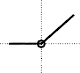
\includegraphics[width=1cm]{./images/bode-approx-ampl-5.png}} &
		\begin{tabular}{ll}
			$\omega < \alpha$: & Konstant $0dB$ \\
			$\omega > \alpha$: & $+20dB/Dek.$
		\end{tabular} &
		\parbox[c][1cm]{1cm}{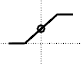
\includegraphics[width=1cm]{./images/bode-approx-phase-5.png}} &
		\begin{tabular}{ll}
			$\omega < \frac{\alpha}{10}$: & Konstant $0$ \\
			$\omega > 10 \alpha$: & Konstant $+\frac{\pi}{2}$
		\end{tabular}
	\\ \hline
		Konjugiert-komplexe Pole \newline
    für $|q_p| > 1/2$ &
		$\frac{1}{s^2+s\frac{\omega_p}{q_p}+\omega_p^2}$ &
		\parbox[c][1cm]{1cm}{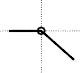
\includegraphics[width=1cm]{./images/bode-approx-ampl-6.png}} &
		\begin{tabular}{ll}
			$\omega < \omega_p$: 	& Konstant $-40 \log \omega_p$ \\
			$\omega > \omega_p$:	& $-40dB/Dek.$ \\
			Überhöhung: 			& $\frac{\omega_p}{2}$ bis $2\omega_p$ \\
			Maximum:				& $-40\log\omega_p + 20 \log q_p$ bei $\omega = \omega_p$			
		\end{tabular} &
		\parbox[c][1cm]{1cm}{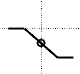
\includegraphics[width=1cm]{./images/bode-approx-phase-6.png}} &
		\begin{tabular}{ll}
			$\omega < \frac{\omega_p}{10^{\frac{1}{2q_p}}}$:	& Konstant $0$ \\
			$\omega > \omega_p 10^{\frac{1}{2q_p}}$:			& Konstant $-\pi$ \\
			$\omega = \omega_p$:								& $-\frac{\pi}{2}$
		\end{tabular}
	\\ \hline
		Konjugiert-komplexe Pole \newline
    für $|q_p| > 1/2$&
		$\frac{\omega_p^2}{s^2+s\frac{\omega_p}{q_p}+\omega_p^2}$ & 
		\parbox[c][1cm]{1cm}{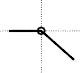
\includegraphics[width=1cm]{./images/bode-approx-ampl-6.png}} &
		\begin{tabular}{ll}
			$\omega < \omega_p$:	& Konstant $0dB$ \\
			$\omega > \omega_p$:	& $-40dB/Dek.$ \\
			Überhöhung:				& $\frac{\omega_p}{2}$ bis $2 \omega_p$ \\
			Maximum:				& $20 \log q_p$ bei $\omega = \omega_p$
		\end{tabular} &
		\parbox[c][1cm]{1cm}{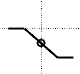
\includegraphics[width=1cm]{./images/bode-approx-phase-6.png}}	& 
		\begin{tabular}{ll}
			$\omega < \frac{\omega_p}{10^{\frac{1}{2q_p}}}$:	& Konstant $0$ \\
			$\omega > \omega_p 10^{\frac{1}{2q_p}}$:			& Konstant $-\pi$ \\
			$\omega = \omega_p$:								& $-\frac{\pi}{2}$
		\end{tabular}
	\\ \hline	
		Konjugiert-komplexe Nullstellen
    für $|q_z| > 1/2$&
		$s^2+s\frac{\omega_z}{q_z}+\omega_z^2$ &
		\multicolumn{4}{l|}{
			Analog zu den Konjugiert-komplexen Polen jedoch gespiegelt an der $0dB$- / $0$-Grad-Linie.
		}
	\\
		&
		$\frac{s^2+s\frac{\omega_z}{q_z}+\omega_z^2}{\omega_z^2}$ &
		\multicolumn{4}{l|}{}
	\\ \hline
		\multicolumn{6}{|p{21cm}|}{
			Serieschaltung von Systemen erfolgt durch \textbf{Superposition} der einzelnen Bode-Diagramme 
			(Multiplikation von UTFs entspricht Addition im	dB-Bereich). $\alpha , \beta \in \mathbf{R}$. 
      Für $\omega_p$ und $q_p$ siehe Kapitel\ref{Polfrequenz Polguete}
		}
	\\ \hline
\end{longtable}
\renewcommand{\arraystretch}{\arraystretchOriginal}
\end{landscape}	